% !TeX spellcheck = en_US
\documentclass{article}


\usepackage{lipsum}
\usepackage[margin=1in,includefoot]{geometry}
\usepackage{graphicx}
\usepackage{float}
\usepackage[hidelinks]{hyperref}
\usepackage{amsmath}
\usepackage{amssymb}
\usepackage{color}
\usepackage[english]{babel}
\usepackage{subcaption}

\usepackage{booktabs}
\usepackage[normalem]{ulem}
\useunder{\uline}{\ul}{}

\usepackage[usenames,dvipsnames]{xcolor}
\usepackage{listings}


% Header and Footer Stuff
\usepackage{fancyhdr}
\pagestyle{fancy}
\fancyhead{}
\fancyfoot{}
\fancyfoot[R]{\thepage}
\renewcommand{\headrulewidth}{0pt}
\renewcommand{\footrulewidth}{0pt}




\definecolor{dkgreen}{rgb}{0,0.6,0}
\definecolor{gray}{rgb}{0.5,0.5,0.5}
\definecolor{mauve}{rgb}{0.58,0,0.82}


\lstset{
 language=C++,
 aboveskip=3mm,
 belowskip=3mm,
 showstringspaces=false,
 columns=flexible,
 basicstyle={\small\ttfamily},
 numbers=none,
 numberstyle=\tiny\color{gray},
 keywordstyle=\color{blue},
 commentstyle=\color{dkgreen},
 stringstyle=\color{mauve},
 breaklines=true,
 breakatwhitespace=true,
 tabsize=3
}




\begin{document}


\begin{titlepage}
	\begin{center}
	\begin{align*}
	
\includegraphics[height=1.75in]{logo.png}
	\end{align*}
	
	\line(1,0){300}\\
	[0.25in]
	\huge{\bfseries Door Detection}\\
	[2mm]
	\line(1,0){200}\\
	[1.5cm]
	\textsc{\LARGE Assignment 2}\\
	[0.75cm]
	\textsc{\Large CS4053 Computer Vision}\\
	[7cm]	
	\end{center}
	
	\begin{flushright}
	\textsc{\large Alexandru Sulea\\
	D Stream\\
	\#12315152\\
	13 December 2016\\}
	\end{flushright}
	
\end{titlepage}
%Table of Contents Stuff%
\tableofcontents
%\listoffigures
%\addcontentsline{toc}{section}{List of Figures}
\listoftables
\addcontentsline{toc}{section}{List of Tables}

\thispagestyle{empty}
\cleardoublepage
\pagenumbering{arabic}
\setcounter{page}{1}

\pagebreak
\section{Intro}\label{sec:intro}
The following lab was based on the procedure of determining when a door is opened and closed in a room given that there is a person walking through the door and that the light in the scene can vary depending on the lighting conditions in the room but also from the light propagating from other sources.\\
The lab was thus conducted with the objective of detecting a door and identifying when said door closes and opens with respect to time as defined in frames.\\

\begin{lstlisting}




\end{lstlisting}
\section{Procedure}\label{sec:intro}
Taking notes of what was discussed and shown in class together with the theory and description on the official Open CV page, the following procedure was planned out. 
The scene itself consists of two distinct parts. The first being a man walking from foreground to background and back, the second being that a door opens and closes at arbitrary intervals. The person in the picture serves no real purpose for this lab other than to induce uncertainty of when the door opens and closes. Thus the first operation is to perform a background subtraction on the person and have them removed as much as possible from the scene. This will not only allow us to see the door more clearly, but it will also help clean up the frames and make Hough Lines more accurate later on.\\


Once the person is removed from the picture, the door detection must begin.\\ Here a number of already built in Open CV procedures can be used such as HoughLines() , HoughLineP() or Line Segment Detector. Although LSD is somewhat more accurate then HoughLineP(), the later is also more easily customizable and faster to process. Given how door frame tracking throughout every video frame was not the objective and only opening and closing, HoughLineP() was chosen to help with the door detection. \\
Here whatever lines were detected in the scene by HoughlinesP(), only the lines that were horizontal or vertical, given 10 degrees of error were accepted as the true vertical and horizontal lines.\\
After the horizontal and vertical lines were filtered through, their determinate is calculated and compared to all the other vertical or horizontal lines as to check if the lines form a box at any point. Should the lines intersect, a circle is drawn at the intersection points.\\
Then a diagonal line is searched for, its point calculated as well as its determinate. Should the diagonal line intersect one of the points where the horizontal and vertical lines intersect, then this is assumed to top side of the door opening, thus creating an angled line.\\ 

The steps for  creating the solution were as follows:\\

The video file is first loaded in to MOG2 which is a background subtraction method, MOG2 was used over MOG due to MOG2 being more adaptable to changing light conditions and also to covering more of the subject with the mask.\\

A bitwise not is then performed on the mask so as to turn it into a foreground subtraction method. This way anything that moves in the foreground is made invisible while the background is largely unaffected The learning rate for the method was chosen at $0.005$ . This was found to have the perfect balance between making the subject invisible, while at the same time keeping the moving door as part of the background.\\




\begin{figure}[H]
\begin{subfigure}{0.5\textwidth}
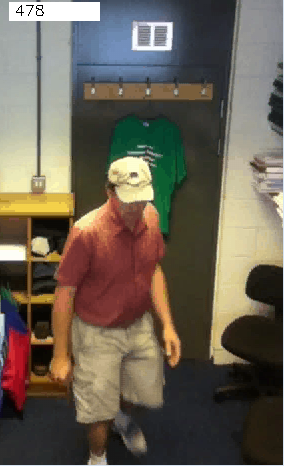
\includegraphics[width=0.5\linewidth, height=5cm]{prof_color.png} 
\caption{unaltered image}
\label{fig:subim1}
\end{subfigure}

\caption{Figure of normal color frame}
\label{fig:image2}
\end{figure}

\begin{lstlisting}
			pMOG2->apply(frame_vid_N, fgMaskMOG2, 0.005);
bitwise_not(fgMaskMOG2, fgMaskMOG2);
absdiff(frame_vid_N, fgMaskMOG2, vid_ands);
//imshow("wvvb", vid_ands);
\end{lstlisting}

Following this procedure, the image was ready to be converted to be able to accept HoughLinesP(). To produce the desired lines, the image was converted to gray scale, so as to be easier to perform adaptive thresholding. Adaptive thresholding was chosen due to its adaptability in varying light conditions. A binary picture was then received which needed to be blurred somewhat to regain some of the lost line continuity. The picture was now ready to be inserted into canny for border detection and then converted back to BGR so as to be able to be combined with other images.

\begin{lstlisting}
cvtColor(frame_vid_N, frame_grey, CV_BGR2GRAY);
adaptiveThreshold(frame_grey, frame_g_tresh, 75, ADAPTIVE_THRESH_GAUSSIAN_C, CV_THRESH_BINARY, 13, 4);
GaussianBlur(frame_g_tresh, frame_blur, Size(5, 5), 1, 1, 1);
Canny(frame_blur, dst, 50, 200, 3);
cvtColor(dst, cdst, COLOR_GRAY2BGR);

\end{lstlisting}






\begin{figure}[H]
	\begin{subfigure}{0.5\textwidth}
		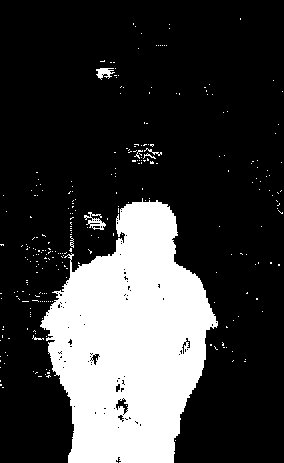
\includegraphics[width=0.5\linewidth, height=5cm]{door_mask.PNG} 
		\caption{MOG2}
		\label{fig:subim1}
	\end{subfigure}
	\begin{subfigure}{0.5\textwidth}
		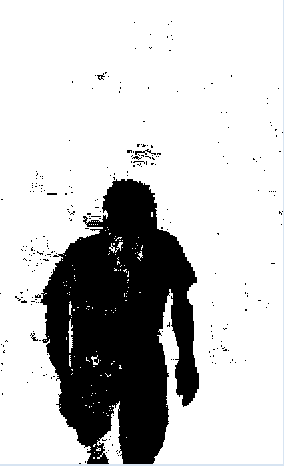
\includegraphics[width=0.5\linewidth, height=5cm]{door_neg_mask.PNG}
		\caption{bitwise not MOG2}
		\label{fig:subim2}
	\end{subfigure}
	\caption{Masks created from background segregation}
	\label{fig:image2}
\end{figure}



\begin{figure}[H]
\center
\begin{subfigure}{0.5\textwidth}
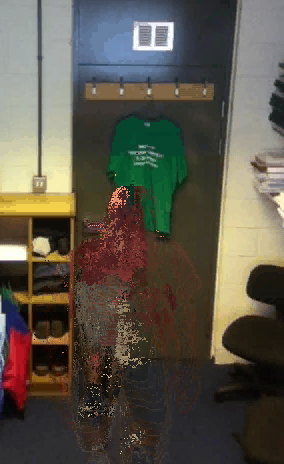
\includegraphics[width=0.5\linewidth, height=5cm]{door_back_proj.PNG} 
\caption{given result of MOG2}
\label{fig:subim1}
\end{subfigure}
\caption{foreground is now transparent}
\label{fig:image2}
\end{figure}


\begin{lstlisting}
	HoughLinesP(dst, lines4, 1, CV_PI / 180, 80+60, 50, 50);
	int vert_line_count = 0;
	int hor_line_count = 0;
	
\end{lstlisting}


\begin{figure}[H]
\begin{subfigure}{0.5\textwidth}
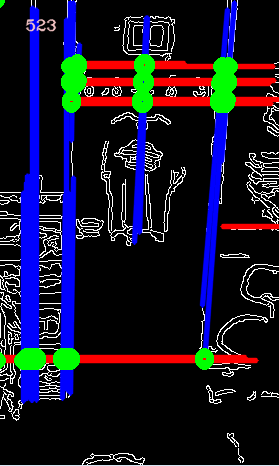
\includegraphics[width=0.5\linewidth, height=5cm]{door_closed_h_v.PNG} 
\caption{video 2 door houghlinesp}
\label{fig:subim1}
\end{subfigure}
\begin{subfigure}{0.5\textwidth}
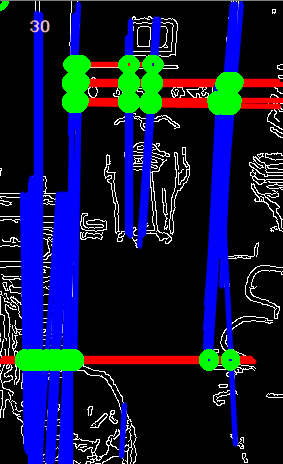
\includegraphics[width=0.5\linewidth, height=5cm]{door2_h_v.PNG}
\caption{video 1 door houghlinesp}
\label{fig:subim2}
\end{subfigure}
\caption{houghlinep}
\label{fig:image2}
\end{figure}


The code below performs a simple detection of houghlinesP given their angles. Thus only the horizontal , vertical and in specific cases, diagonal lines are stored. The code below shows how this was achieved. All code was sourced from basic calculus with the exception of the intersection algorithm which was taken from an opencv online tutorial.

\begin{lstlisting}
for (size_t i = 0; i < lines4.size(); i++)
{
Vec4i l = lines4[i];
/*get angle of line*/
double angle = atan2(l[3] - l[1], l[2] - l[0]) * 180 / CV_PI;
\end{lstlisting}
Code above runs a loop for every line detected in the frame. with the help of houghlineP detection we know that the number of lines detected is lines4.size(). The angle is then calculated through basic calculus and then converted to degrees as atan2() gives an answer in radians.


\begin{lstlisting}

/*horizontal lines*/
if (angle <5 && angle >= -5 || angle <-175 && angle >= 175)
{
hor_line_count++;
h_l.push_back(l);
//cout << "HORIZONTAL LINES " <<Point(l[0],l[1])<<Point(l[2],l[3]) <<endl;
line(cdst, Point(l[0], l[1]), Point(l[2], l[3]), Scalar(0, 0, 255), 3, CV_AA);
}
/*vertical lines */
if (angle< 95 && angle >= 85 || angle < -85 && angle >= -95)
{
vert_line_count++;
v_l.push_back(l);
//cout << "VERTICAL LINES " << Point(l[0], l[1]) << Point(l[2], l[3]) << endl;
line(cdst, Point(l[0], l[1]), Point(l[2], l[3]), Scalar(255, 0, 0), 3, CV_AA);		
}

\end{lstlisting}
The code above filters all the lines detected in the frame and only gives the points of the lines which are horizontal or vertical  $\pm{5}$ degrees. This is done in an effort to find the door frames. Since most standard doors have exclusively horizontal and vertical edges, it is then safe to assume that searching for those edges will identify a door, among other objects.\\


\begin{lstlisting}


/*if door not closed*/
if (angle <-5 && angle >= -25 || angle <175 && angle >= 150 || angle >-175 && angle <= -150)
{
if (frame_thresh > frame_count - last_frame) {
open_close_count++;
oc_l.push_back(l);
//cout << "DIAGONAL LINES " << Point(l[0], l[1]) << Point(l[2], l[3]) << "FRAME " << frame_count << endl;
}


\end{lstlisting}
The above code filters and counts the diagonal lines. These lines will help identify our door as a door. Even tho most objects in the world are square in shape, very few can make a diagonal line with what was once a horizontal one. This phenomenon is exclusive to a plane rotating either to or from the camera, but the edge rotating away from view and the edge rotating towards the view will create a diagonal line. Thus providing a means to identify doors.\\
\begin{lstlisting}

else {
last_frame = frame_count;
diag_line_count++;
diag_l.push_back(l);
line(cdst, Point(l[0], l[1]), Point(l[2], l[3]), Scalar(0, 200,200), 3, CV_AA);
if (diag_line_count % 2 == 0) {
cout << "Door Closes on points " << Point(l[0], l[1]) << Point(l[2], l[3]) << " at FRAME " << frame_count << endl;
}
else {
cout << "Door Opens on points " << Point(l[0], l[1]) << Point(l[2], l[3]) << " at FRAME " << frame_count << endl;
}
}}}
/*Draw circle at line intersection*/
for (int i = 0; i < h_l.size(); i++)
{
for (int j = 0; j < v_l.size(); j++)
{
Point poi = intersection(Point(h_l[i][0], h_l[i][1]), Point(h_l[i][2], h_l[i][3]), Point(v_l[j][0], v_l[j][1]), Point(v_l[j][2], v_l[j][3]));
circle(cdst, poi, 6, Scalar(0, 255, 0),  5,  8,0);
}}

\end{lstlisting}
Once the horizontal, diagonal and vertical lines have been detected the filter in the code above will find the points of intersection from the vertical and horizontal and draw them.\\

\begin{lstlisting}


for (int i = 0; i < h_l.size(); i++)
{
for (int j = 0; j < oc_l.size(); j++)
{
Point poi = intersection(Point(h_l[i][0], h_l[i][1]), Point(h_l[i][2], h_l[i][3]), Point(oc_l[j][0], oc_l[j][1]), Point(oc_l[j][2], oc_l[j][3]));
if ( (Point(h_l[i][0], h_l[i][1]) == Point(oc_l[j][0], oc_l[j][1])) || (Point(h_l[i][2], h_l[i][3]) == Point(oc_l[j][2], oc_l[j][3])) || (Point(h_l[i][2], h_l[i][3]) == Point(oc_l[j][0], oc_l[j][1])) || (Point(h_l[i][0], h_l[i][1]) == Point(oc_l[j][2], oc_l[j][3])) )
{
line(cdst, Point(oc_l[i][0], oc_l[i][1]), Point(oc_l[i][2], oc_l[j][3]), Scalar(0, 200, 200), 3, CV_AA);
circle(cdst, poi, 6, Scalar(200, 0, 200), 5, 8, 0);
}}}

\end{lstlisting}
Those intersecting points are then compared with any diagonal line points that may intersect them. This will lead to the horizontal line turning into the diagonal line as discussed above. Once these lines appear, they are stored and counted. Due to watching the video we know that there are 2 sets of door opening and closing. Furthermore we know that a door cant possibly open and close within 50 frames. Thus a count is implemented to accurately detect the diagonal line when it appears but also to filter out any line repeats that may occur due to thresholding induced defects.




\section{Performance}\label{sec:intro}
Given as how the ground truth was provided or this lab in terms of door frame position and opening and closing frames, it was quite simple to compare the achieved results to the ground truth. \\

As can be seen from the scores below, the algorithm performs quite well in detecting when the door opens and closes. The algorithm begins to loose accuracy in the variable light image and also in the larger pictures.\\
This problem is two fold and its causes are also independent of each other. The inaccuracy from the variable light is due to the light distorting the binary outputs of the MOG2 and also the adaptive thresholding. While it is advertised that adaptive thresholding is adaptive in variable light, this has its limits and is not a complete solution. Too much thresholding can lead to loosing important features, while too little thresholding can lead to unwanted error inducing details.\\
The larger video is less accurate due to it having a more clear picture of the objects in it. These objects are harder to threshold out during the process and thus will induce errors when processing the video.\\
The higher the video quality, the higher the pixel density , thus while higher definition videos are generally more preferred, these videos take far longer to process or demand faster and more expensive hardware.\\


\begin{figure}[H]
	\begin{subfigure}{0.5\textwidth}
		\includegraphics[width=1\linewidth, height=5cm]{door2_score.PNG} 
		\caption{door video 1 score}
		\label{fig:subim1}
	\end{subfigure}
	\begin{subfigure}{0.5\textwidth}
		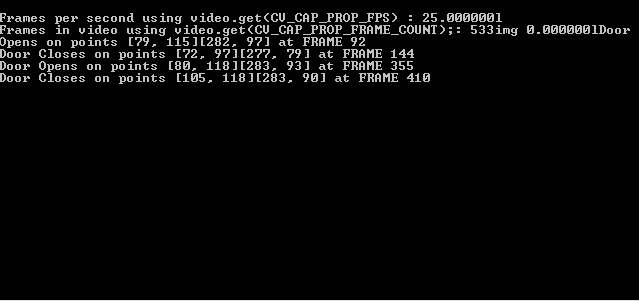
\includegraphics[width=1\linewidth, height=5cm]{door1_score.PNG}
		\caption{door video 2 score}
		\label{fig:subim2}
	\end{subfigure}
	\caption{Scores for door video 3 and 4}
	\label{fig:image2}
\end{figure}



\begin{figure}[H]
	\begin{subfigure}{0.5\textwidth}
		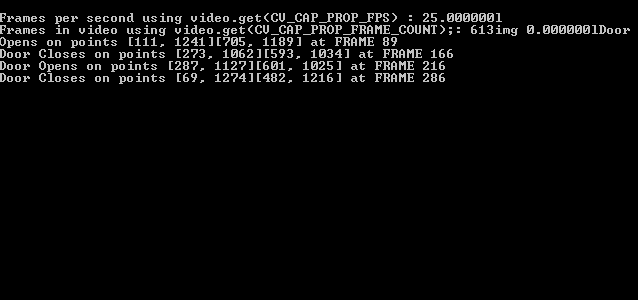
\includegraphics[width=1\linewidth, height=5cm]{door3_score.PNG} 
		\caption{door video 3 score}
		\label{fig:subim1}
	\end{subfigure}
	\begin{subfigure}{0.5\textwidth}
		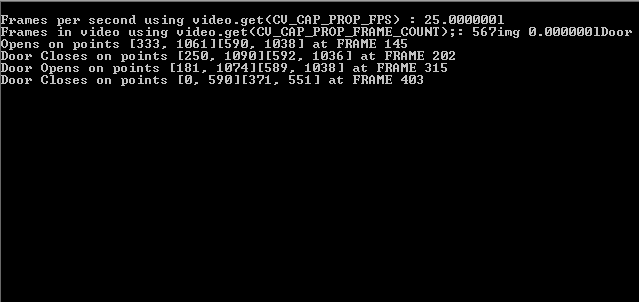
\includegraphics[width=1\linewidth, height=5cm]{Door44_score.PNG}
		\caption{door video 4 score}
		\label{fig:subim2}
	\end{subfigure}
	\caption{Scores for door video 3 and 4}
	\label{fig:image2}
\end{figure}

\begin{table}[H]
	\centering
	\caption{Recorded Results}
	\label{my-label}
	\begin{tabular}{|l|l|l|l|l|}
		\hline
		Video & 1st Door Open Frame & 1st Door Close Frame & 2nd Door Open Frame & 2nd Door Close Frame     \\ \hline
		1                     & 104                  & 164            & 378               & 458 \\ \hline
		2                     & 92                  & 144            & 355             & 410\\ \hline
		3                     & 89                     & 166                    & 216                     & 286 \\ \hline
		4                     & 51                     & 107                    & 157                     & 315 \\ \hline
	\end{tabular}
\end{table}

\begin{table}[H]
	\centering
	\caption{Ground truth}
	\label{my-label}
	\begin{tabular}{|l|l|}
		\hline
		First open close & Second open close \\ \hline
		94-211           & 373-490           \\ \hline
		71-184           & 339-460           \\ \hline
		153-251          & 380-492           \\ \hline
		134-230          & 311-432           \\ \hline
	\end{tabular}
\end{table}


\section{Discussion}\label{sec:intro}
While solving the problems inherent in detecting a door, a number of problems arose. The main being that, even though the solution was designed to fit a wide array of cases, it will fail in many more due to a variety of problems such as:

\begin{enumerate}
	\item The precision and accuracy of the solution is heavily dependent of the lighting conditions present and also the color difference of the door as opposed to its background.\\ While doing the lab, algorithms continually had problems detecting where the door ended and the door frame ended, due to the fact that the two were very flush and of the same design and color.
	\item The door shape itself would need to have 4 corners to provide an accurate door representation, any lift doors or star trek/ star wars type doors would not be detected. 
	
	\item The next group of problems arise once the video is recorded of a viable door opening and closing Assuming that the door conforms to the standard door dimensions and that the video angle is not skewed then the question of lighting comes into effect. Too much or little light, such as when a powerful lamp is turned on or when the lights are off can seriously effect the accuracy of the algorithm. One option to offset this issue is to use infra red enabled cameras so as to get a more light independent picture.
	
	\item Even if a door is detected, the continual detection of the door will depend on a clear line of sight from the camera to the door and also a preferably higher definition image for improved accuracy. People or objects existing between the camera and door line of sight can seriously hamper the accuracy. Thus to mitigate this effect, a back projection algorithm is generally advised.
	
	
\end{enumerate}


The problems outlined above are just the general outline. There are many more problems which may be case specific. In manual doors for example, a door opening or closing at an uneven rate can also decrease the accuracy and precision of the door detection.\\
Lastly there are the accuracy errors which were due to false positives and false negatives in the video.\\
The false positives were mostly due to noise in the original video, which through thresholding and canny promulgated in the HoughLines video. This was easy to fix by adjusting the thresholding of the video to a value at which there was a minimum amount of error but still enough detail for lines to be drawn.\\
Light reflectance was found to be a major cause of the earliest false positives. As the door is not mat but glossy. This property combined with light shining directly on the door cause the door to somewhat reflect the objects in front of it but behind the camera. Giving the impression that the door may be moving, when in fact it is static.


The false negatives were somewhat harder to solve as important details in the video may be lost through canny. Thus a line that existed and was clearly defined in the color, unaltered version of the video may have dissipated. This can be somewhat corrected by extending or merging lines in the HoughLinesP() function, although this does not work for all cases. \\

Lastly, the solution presented does not solve for all cases. One example may be that if a door is continuously rocked back and forth. Such as in a busy hallway where someone may hold the door for many other people. The algorithm will see the back and forth movement of the door as opening and closing. As there is no state of a door being opened. Only that a door is about to be opened or about to be closed.\\









\pagebreak
\end{document}


